% LaTeX file for resume
\documentclass[11pt,a4paper, french]{article}
\usepackage[francais]{babel}
\usepackage[utf8]{inputenc}
\usepackage{amsmath}
\usepackage{amsfonts}
\usepackage{amssymb}


\usepackage[usenames, dvipsnames]{xcolor}

\usepackage[framemethod=tikz]{mdframed}
\newmdenv[innerlinewidth=0.8pt, roundcorner=4pt,linecolor=RoyalBlue,innerleftmargin=6pt,
innerrightmargin=6pt,innertopmargin=6pt,innerbottommargin=6pt]{mybox}
\usepackage{wrapfig}


\usepackage{etaremune}

\definecolor{gris}{rgb}{0.45,0.45,0.45}
\definecolor{blanc}{rgb}{1,1,1}

\usepackage[colorlinks = true,urlcolor = BrickRed]{hyperref}

\usepackage{eurosym}


\usepackage{datetime}
\newdateformat{monthyeardate}{%
  \monthname[\THEMONTH] \THEYEAR}

\usepackage{fancyhdr}  % use this package to get a 2 line header
\renewcommand{\headrulewidth}{0pt} % suppress line drawn by default by fancyhdr

\setlength{\headsep}{0pt}  % space between header and text
% \setlength{\footskip}{2pt}
\pagestyle{fancy}     % set pagestyle for document

\rhead{\textcolor{gris}{ \thepage/9}}
\chead{\textcolor{gris}{}} % put text in header (right side)
\cfoot{}
\lfoot{\textcolor{Gray}{CV mis à jour en \monthyeardate\today}}

% \lfoot{\textcolor{Gray}{CV mis à jour en \monthyeardate\today}}
\rfoot{\href{http://johanmazoyer.com}{johanmazoyer.com}}


\setlength{\parindent}{0pt}

\setlength{\headwidth}{17.2cm} % taille de l'entete
\usepackage[total={17.2cm,25.cm}, left=1.9cm, top=2.5cm]{geometry}

\begin{document}

\lhead[]{}
\begin{huge}
\noindent\textbf{Johan MAZOYER}
\end{huge}\\

\textbf{Interêts de recherche:} Instrumentation Optique, Imagerie Directe et Coronographie,
Observation et Charactérisation de Systèmes Extrasolaires, Disques de Débris\\



%%%%%%%%%%%%%%%%%%%%%%%%%%%%%%%%%%%%%%%%%%%%%%%%%%%%%%%%%%%%%%%%%%%%%%%%%%%%%%%%%%%%%%%%%%%%%%%%%%%%%%%%%%%%%%%%%%%%%%%%
%%%%%% SECTION RESEARCH EXPERIENCE
%%%%%%%%%%%%%%%%%%%%%%%%%%%%%%%%%%%%%%%%%%%%%%%%%%%%%%%%%%%%%%%%%%%%%%%%%%%%%%%%%%%%%%%%%%%%%%%%%%%%%%%%%%%%%%%%%%%%%%%%


\vspace{-0.8cm}
\textcolor{RoyalBlue}{\section{\large EXPÉRIENCES PROFESSIONNELLES}
\vspace{-0.2cm}\hrule}
\vspace{0.4cm}


\textbf{Chargé de recherche CNRS} --
\href{http://www.obspm.fr}{\textbf{LESIA / Observatoire de Paris}}
\hfill     	 { \bf starting 2020}\\

\vspace{-0.05cm}
\textbf{Carl Sagan Postdoctoral Fellow} --
\href{https://www.jpl.nasa.gov/}{\textbf{Jet Propulsion Laboratory}}
\hfill      { \bf 2018 - 2019}\\

\vspace{-0.05cm}
\textbf{Chercheur post-doctoral} --
\href{http://physics-astronomy.jhu.edu/}{\textbf{Johns Hopkins University}}
\hfill   	 { \bf 2016 - 2018}\\

\vspace{-0.05cm}
\textbf{Chercheur post-doctoral} --
{\href{http://www.stsci.edu}{\textbf{Space Telescope Science Institute}}}
\hfill        { \bf 2014 - 2016}\\\

\vspace{-0.05cm}
\textbf{Doctorant} --
\href{http://www.obspm.fr/?lang=en}{\textbf{LESIA/Paris Observatory}}
\hfill        { \bf 2011 - 2014}\\


% \textbf{Jet Propulsion Laboratory} (JPL)  \hfill       {\small Pasadena, CA, USA} \\
% {\small \textit{Carl Sagan Fellow}}  \hfill  	 {\small \bf 2018 -- Présent}\\

% \vspace{-0.2cm}
% \hspace{0.5cm} \parbox{0.9\linewidth}{
%    \begin{itemize} \itemsep -3pt % reduce space between items
%    \vspace{-0.4cm}
%     \item \small Astrophysique : Caractérisation de disques avec GPI et WFIRST
%    \item \small Instrumentation : Développement de techniques instrumentales sur banc optique
%  \end{itemize} }\\

% \textbf{Johns Hopkins University} (JHU) \hfill       {\small Baltimore, MD, USA} \\
% {\small \textit{Chercheur post-doctoral}; superviseur : Christine Chen}  \hfill  	 {\small \bf 2016 -- 2018}\\

% \vspace{-0.4cm}
% \hspace{0.5cm} \parbox{0.9\linewidth}{
%    \begin{itemize} \itemsep -3pt % reduce space between items
%    \vspace{-0.2cm}
%     \item \small Astrophysique : Large programme sur les disques de débris sur GPI
%    \item \small Instrumentation : Méthodes deux miroirs pour l'imagerie haut-contraste
%  \end{itemize} }\\

% \vspace{-0.2cm}
% \textbf{Space Telescope Science Institute} (STScI) \hfill       {\small Baltimore, MD, USA} \\
% {\small \textit{Chercheur post-doctoral}; superviseur : Laurent Pueyo}  \hfill  	 {\small \bf 2014 --2016}\\

% \vspace{-0.4cm}
% \hspace{0.5cm} \parbox{0.9\linewidth}{
%    \begin{itemize} \itemsep -3pt % reduce space between items
%    \vspace{-0.2cm}
%     \item \small Astrophysique : Imagerie directe de disques (NICMOS, NICI, SPHERE)
%    \item \small Instrumentation : Correction active d'ouvertures de télescopes complexes \\

%  \end{itemize} }

% \vspace{-0.2cm}
% \textbf{Laboratoire d'études spatiales et d'instrumentation en astrophysique} (LESIA)  \hfill        {\small Paris, FR} \\
% {\small \textit{Doctorant}; encadrants : Pierre Baudoz et Gérard Rousset}  \hfill  	 	 {\small \bf 2011 -- 2014}\\
% \vspace{-0.1cm}
% \hspace{0.5cm} \parbox{0.9\linewidth}{
% \vspace{0.2cm}
% \small  Développement d'un senseur de front d'onde haut-contraste et imagerie\\ de disques de débris (Gemini/NICI)} \\

% \vspace{0.2cm}
% \textbf{Los Alamos National Laboratory} (LANL) \hfill    	Los Alamos, NM, USA\\
% {\small \textit{Étudiant de M2}; encadrants : Roger C. Wiens et Jérémie Lasue
%  \hfill  		 {\bf 2011}}\\
%  \vspace{-0.4cm}
% \hspace{0.5cm} \parbox{0.9\linewidth}{
% \small  MSL/ChemCam : Influence de l'atmosphère martienne sur les limites de détection} \\

% \vspace{0.1cm}
% \textbf{Institut de Recherche en Astrophysique et Planétologie} (IRAP) \hfill    	Toulouse, FR\\
% {\small \textit{Étudiant de M2}; encadrants:  Sylvestre Maurice et Olivier Gasnault
%  \hfill  		 {\bf 2011}}\\
%  \vspace{-0.4cm}
% \hspace{0.5cm} \parbox{0.9\linewidth}{
% \small  MSL/ChemCam : Influence de l'atmosphère sur les mesures du LIBS} \\

%\vspace{0.1cm}
% \textbf{CNES} \hfill    	Toulouse, France\\
%{\small \textit{Étudiant de M1}; Satellites Pleiades : simulation de composants de vol\hfill  		 {\bf Mars -- Juil. 2010}}\\
%
%\vspace{-0.3cm}
%\textbf{Le Relais} (Emmaüs) \hfill    		  Koudougou, Burkina Faso\\
%{\small Stage humanitaire\hfill  		  {\bf Juil. -- Sept. 2009}}	\\

%%%%%%%%%%%%%%%%%%%%%%%%%%%%%%%%%%%%%%%%%%%%%%%%%%%%%%%%%%%%%%%%%%%%%%%%%%%%%%%%%%%%%%%%%%%%%%%%%%%%%%%%%%%%%%%%%%%%%%%%
%%%%%% SECTION EDUCATION
%%%%%%%%%%%%%%%%%%%%%%%%%%%%%%%%%%%%%%%%%%%%%%%%%%%%%%%%%%%%%%%%%%%%%%%%%%%%%%%%%%%%%%%%%%%%%%%%%%%%%%%%%%%%%%%%%%%%%%%%

\vspace{-0.3cm}
\textcolor{RoyalBlue}{\section{\large FORMATION}
\vspace{-0.2cm}\hrule}
\vspace{0.4cm}

{\sl Doctorat}, \href{https://www.univ-paris-diderot.fr/}{\textbf{Universit\'e Paris Diderot}}
\hfill Paris, France\\
Astronomie et Astrophysique \hfill  {\small \bf Septembre 2014}\\

\vspace{-0.05cm}
{\sl Master 2},
\href{http://ezomp2.omp.obs-mip.fr/asep/index.php/eng}{\textbf{Université Paul Sabatier} }
 \hfill Toulouse, France\\
Astrophysique, Science de l'Espace, Planétologie \hfill {\small \bf Septembre 2011}\\

\vspace{-0.05cm}
{\sl Diplôme d'ingénieur}, \href{https://www.isae-supaero.fr/en/}{\textbf{\textbf{ISAE Supaero} }}  \hfill Toulouse, France\\
Systèmes Spatiaux et Techniques d'Imageries Spatiales \hfill  {\small \bf Septembre 2011} \\


\vspace{-0.05cm}
{\sl Diplôme d'ingénieur}, \href{http://www.polytechnique.edu/en/}{\textbf{\textbf{Ecole polytechnique} }}
\hfill Paris, France  \\
Systèmes Embarqués (électronique et informatique)  \hfill {\small \bf Septembre 2011}\\

%%%%%%%%%%%%%%%%%%%%%%%%%%%%%%%%%%%%%%%%%%%%%%%%%%%%%%%%%%%%%%%%%%%%%%%%%%%%%%%%%%%%%%%%%%%%%%%%%%%%%%%%%%%%%%%%%%%%%%%%
%%%%%% SECTION AWARDS
%%%%%%%%%%%%%%%%%%%%%%%%%%%%%%%%%%%%%%%%%%%%%%%%%%%%%%%%%%%%%%%%%%%%%%%%%%%%%%%%%%%%%%%%%%%%%%%%%%%%%%%%%%%%%%%%%%%%%%%%

\vspace{-0.3cm}
\textcolor{RoyalBlue}{\section{\large BOURSES \& PRIX}
\vspace{-0.2cm}\hrule}
\vspace{0.4cm}

\textbf{Carl Sagan Fellowship}  \hfill   2018\\

\vspace{-0.15cm}
Couverture du journal \textbf{Astronomy \& Astrophysics} (Volume 564) \hfill  2014\\

\vspace{-0.15cm}
\textbf{Meilleure présentation}, conférence des chercheurs du CNES (JC2) \hfill   2013\\

\vspace{-0.15cm}
\textbf{Bourse de recherche} du CNES \hfill   2011\\

\vspace{-0.15cm}
\textbf{Bourse d'étude} de l'Ecole polytechnique \hfill   2007\\

%%%%%%%%%%%%%%%%%%%%%%%%%%%%%%%%%%%%%%%%%%%%%%%%%%%%%%%%%%%%%%%%%%%%%%%%%%%%%%%%%%%%%%%%%%%%%%%%%%%%%%%%%%%%%%%%%%%%%%%%
%%%%%% SECTION VULGARISATION
%%%%%%%%%%%%%%%%%%%%%%%%%%%%%%%%%%%%%%%%%%%%%%%%%%%%%%%%%%%%%%%%%%%%%%%%%%%%%%%%%%%%%%%%%%%%%%%%%%%%%%%%%%%%%%%%%%%%%%%%

% \newpage
% \textcolor{blanc}{.}
\vspace{-0.3cm}
\textcolor{RoyalBlue}{\section{\large DIFFUSION DES SCIENCES}
\vspace{-0.2cm}\hrule}
\vspace{0.4cm}
\begin{wrapfigure}{r}{0.23\textwidth}
\vspace{-0.8cm}
\begin{mybox}
    
\includegraphics[width=1.\textwidth]{figures_CV/PodcastScience.png}
 \end{mybox}
\vspace{-0.8cm}
\end{wrapfigure}
\textbf{Podcast Science} \\
\vspace{-0cm}
\hspace{0.3cm}
J'anime chaque semaine \href{http://www.podcastscience.fm}{PodcastScience.fm},
\textbf{émission scientifique hebdomadaire de radio} (podcast) d'une heure et demie à
3h. Le podcast produit des émissions sur tous les domaines scientifiques et je réalise tous les contenus
relatifs à la physique et à l'astrophysique.

\vspace{0.4cm}
\textbf{Conférences grand public}   \\
\hspace{0.3cm} CERN (Genève) et Palais de la découverte (Paris)\\




%%%%%%%%%%%%%%%%%%%%%%%%%%%%%%%%%%%%%%%%%%%%%%%%%%%%%%%%%%%%%%%%%%%%%%%%%%%%%%%%%%%%%%%%%%%%%%%%%%%%%%%%%%%%%%%%%%%%%%%%
%%%%%% SECTION TEACHING EXPERIENCE
%%%%%%%%%%%%%%%%%%%%%%%%%%%%%%%%%%%%%%%%%%%%%%%%%%%%%%%%%%%%%%%%%%%%%%%%%%%%%%%%%%%%%%%%%%%%%%%%%%%%%%%%%%%%%%%%%%%%%%%%

\textcolor{RoyalBlue}{\section{\large ENSEIGNEMENT ET ENCADREMENTS}
\vspace{-0.2cm}\hrule}
\vspace{0.4cm}

\textbf{Co-encadrement de doctorants}\\
\vspace{-0.3cm}

\begin{itemize} \itemsep 5pt
    \item[$\bullet$] \textbf{Lucie Leboulleux} (thèse soutenue en Décembre 2018)
    \item[$\bullet$] \textbf{Kevin Fogarty} (thèse soutenue en Août 2017)\\
\end{itemize}
\textbf{Qualification aux fonctions de maître de conférences dans la section 34}\hfill  2015

\vspace{0.3cm}
\textbf{Universit\'e Paris Diderot -- Paris 7} \hfill  		 2013 \& 2014
\begin{itemize} \itemsep 5pt
    \item[$\bullet$] 32h de vacation (électronique pour L3 cursus ingénieur)\\
\end{itemize}

\textbf{Universit\'e Paris Descartes -- Paris 5} \hfill  		 2011 \& 2012
\begin{itemize} \itemsep 5pt
    \item[$\bullet$] 72h de vacation (hydrodynamique pour L1 cursus médecine)\\
\end{itemize}


\textbf{La Main à la pâte -- Académie de Perpignan} \hfill 2007 -- 2008
\begin{itemize} \itemsep 5pt
    \item[$\bullet$] Stage de première année de l'Ecole polytechnique (8 mois) où
     j'ai enseigné les sciences en primaire à temps plein. Les mercredis étaient
     consacrés à la formation des professeurs des écoles à l'enseignement des sciences.
\end{itemize}




%%%%%%%%%%%%%%%%%%%%%%%%%%%%%%%%%%%%%%%%%%%%%%%%%%%%%%%%%%%%%%%%%%%%%%%%%%%%%%%%%%%%%%%%%%%%%%%%%%%%%%%%%%%%%%%%%%%%%%%%
%%%%%% campagnes d’observations
%%%%%%%%%%%%%%%%%%%%%%%%%%%%%%%%%%%%%%%%%%%%%%%%%%%%%%%%%%%%%%%%%%%%%%%%%%%%%%%%%%%%%%%%%%%%%%%%%%%%%%%%%%%%%%%%%%%%%%%%

% \vspace{-0.4cm}
% \textcolor{RoyalBlue}{\section{\large CAMPAGNES D'OBSERVATIONS}
% \vspace{-0.3cm}\hrule}
% \vspace{0.3cm}

% \textbf{Palomar Observatory (200 inch telescope)}
% \begin{itemize} \itemsep -1pt % reduce space between items
% 	    \item \small Mai 2015, 3 nuits -- Premiers tests sur télescope de la Self-Coherent Camera
% \end{itemize}

% \textbf{Gemini South/GPI}
% 	\begin{itemize} \itemsep -1pt % reduce space between items
% 	    \item \small Décembre 2015 - Novembre 2018 --	25 nuits en cumulé pour le large programme disque ou le programme de temps garanti du consortium GPI. Depuis fin 2016, toutes les observations Gemini sud sont menées à distance. J'ai effectué la majorité de mes observations à distance depuis Berkeley, le JPL et le STScI.
% \end{itemize}



%%%%%%%%%%%%%%%%%%%%%%%%%%%%%%%%%%%%%%%%%%%%%%%%%%%%%%%%%%%%%%%%%%%%%%%%%%%%%%%%%%%%%%%%%%%%%%%%%%%%%%%%%%%%%%%%%%%%%%%%
%%%%%% Demandes de temps
%%%%%%%%%%%%%%%%%%%%%%%%%%%%%%%%%%%%%%%%%%%%%%%%%%%%%%%%%%%%%%%%%%%%%%%%%%%%%%%%%%%%%%%%%%%%%%%%%%%%%%%%%%%%%%%%%%%%%%%%

% \newpage
% \textcolor{blanc}{.}
% \vspace{-0.8cm}
% \textcolor{RoyalBlue}{\section{\large DEMANDES DE TEMPS D'OBSERVATION ACCEPTÉES}
% \vspace{-0.3cm}\hrule}
% \vspace{0.3cm}

% \textbf{GEMINI South/GPI} : Membre du consortium GPI depuis septembre 2016
% \vspace{0.3cm}
% \begin{itemize} \itemsep -1pt % reduce space between items
%     \item \small GS-2015B-LP-6 ``Characterizing Dusty Debris in Exoplanetary Systems'' (PI: C. Chen)
%     \item \small DT-2019A-009 ``Decoding the Asymmetric Scattered Light Around HD 15115'' (PI: C. Chen)
%     \item \small GS-2019A-Q-109 ``Completing a Survey for Resolved Debris Disks in the Sco-Cen Assoc.'' (PI: J. Patience)
% \end{itemize}


% \textbf{VLT/SPHERE}
% %\vspace{-0.2cm}
% \begin{itemize} \itemsep -1pt % reduce space between items
% 	\item \small P 0101.C-0128 ``Resolving multiple belts and sub-structures in inner regions of highly inclined debris disks" (PI : A. Boccaletti)
%     \item \small P 098.C-0686 ``Resolving sub-structures in rings and gaps of inclined debris disks" (PI : A. Boccaletti)
%     \item \small P 096.C-0640 ``Exploring the inner cavities of two very inclined debris disks'' (PI : A. Boccaletti)
%     \item \small P 095.C-0381 ``Investigating the inner part of a transitional disk" (PI : A. Boccaletti)
% \end{itemize}

% \textbf{JWST / MIRI, NIRCam, NIRSPEC \& NIRISS}
% %\vspace{-0.2cm}
% \begin{itemize} \itemsep -1pt % reduce space between items
%     \item \small Programme Early realease Science (ERS) ``High Contrast Imaging of Exoplanets and Exoplanetary Systems with JWST" (PI : Sasha Hinkley)
% \end{itemize}

%%%%%%%%%%%%%%%%%%%%%%%%%%%%%%%%%%%%%%%%%%%%%%%%%%%%%%%%%%%%%%%%%%%%%%%%%%%%%%%%%%%%%%%%%%%%%%%%%%%%%%%%%%%%%%%%%%%%%%%%
%%%%%% SECTION RESPONSABILITE
%%%%%%%%%%%%%%%%%%%%%%%%%%%%%%%%%%%%%%%%%%%%%%%%%%%%%%%%%%%%%%%%%%%%%%%%%%%%%%%%%%%%%%%%%%%%%%%%%%%%%%%%%%%%%%%%%%%%%%%%
\vspace{-0.3cm}
\textcolor{RoyalBlue}{\section{\large PRISES DE RESPONSABILITÉS POUR LA COMMUNAUTÉ}
\vspace{-0.2cm}\hrule}
\vspace{0.4cm}
% \lhead{\textcolor{gris}{J. MAZOYER}}

\textbf{Organisation de conférences et ateliers}\\
\vspace{-0.1cm}
% \begin{wrapfigure}{r}{0.4\textwidth}
% \vspace{-1.2cm}
% \begin{mybox}
%     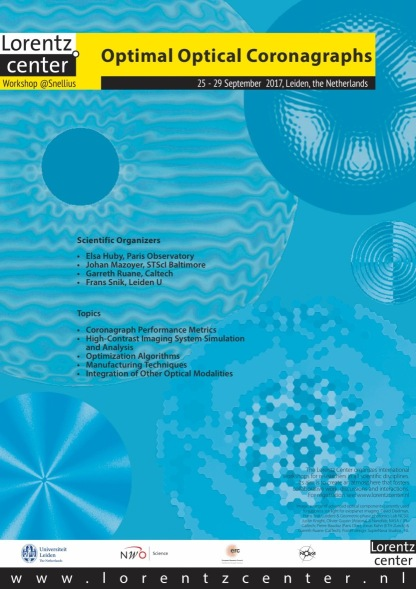
\includegraphics[width=1.\textwidth]{figures_CV/ooc_poster2_sm.jpg}
%  \end{mybox}
% \end{wrapfigure}
% \vspace{-0.2cm}
\begin{itemize} \itemsep 5pt
    \item[$\bullet$] \small Science Organizing Comitee et organisateur de la conference  \textbf{National Capital Area Disks} (Baltimore, MD, Oct. 2018). \href{https://sites.google.com/view/ncad7-at-jhu/ncad7}{\underline{\textbf{Site internet}}}
    \item[$\bullet$] \small Science Organizing Comitee et co-organisateur de l'atelier \textbf{Optimal Optical Coronagraphs (Leiden, NL, Sep. 2017)}. \href{https://www.lorentzcenter.nl/lc/web/2017/924/info.php3?wsid=924&venue=Snellius}{\underline{\textbf{Site internet}}}
    \item[$\bullet$] \small \textit{Science Organizing Comitee} de l'atelier \textbf{High Contrast Imaging from Space (Baltimore, MD, US, Nov 2016)}.  \href{http://www.cvent.com/events/high-contrast-imaging-in-space-workshop/event-summary-eb3bb6bd54a342c5a15678daa49be683.aspx}{\underline{\textbf{Site internet}}}
    \item[$\bullet$] \small Co-organisateur de l'atelier \textbf{La très haute dynamique (Paris, Fr, Oct. 2012)}
\end{itemize}
\vspace{0.4cm}
%\textbf{Développement d'un logiciel pour la communauté}\\
%\vspace{-0.7cm}
%\begin{itemize} \itemsep -3pt % reduce space between items
%    \item \small Développement d'un \textit{pipeline} pour le consortium GPI pour traiter les disques avec l'instrument coronographique GEMINI/GPI. Ce code, dit de \textit{forward-modelling} permettra à terme d'identifier les effets sur la forme et la photométrie dus au traitement d'image.
%\end{itemize}


\textbf{Autres investissements}\\
\vspace{-0.1cm}
\begin{itemize} \itemsep 5pt
    \item[$\bullet$] \small Participation au {\bf Telescope Allocation Committee} d'Hubble (2 semaines, Mai 2016).
    \item[$\bullet$] \small Membre du Study Analysis Groups (SAGs) \#19 de l'\textbf{Exoplanet Exploration Program Analysis Group} (ExoPAG). Le SAG numéro 19 regroupe des chercheurs pour définir de nouvelles métriques d'évaluation et de comparaison des méthodes de détection d'exoplanètes (Jensen Clem et al. 2017).
    \item[$\bullet$] \small Organisation du \textbf{séminaire ``Exoplanet, Star and Planet Formation"} au STScI (2016 - 2018). Ce séminaire invite des chercheurs d'autres organismes chaque semaine au STScI.
    \item[$\bullet$] \small Développement du \textbf{site internet du banc optique THD} de Meudon en Août 2014, dans l'objectif de faire connaître ses caractéristiques à l'international pour créer de nouvelles collaborations.
    \item[$\bullet$] \small \textbf{Peer-review} pour le \textit{Astronomical Journal}, \textit{A\&A}, \textit{MNRAS}, \textit{PASP} et \textit{Journal of Astronomical Telescopes, Instruments, and Systems}.
\end{itemize}

% \vspace{-0.35cm}
% \textcolor{RoyalBlue}{\section{\large REFERENCES}
% \vspace{-0.3cm}\hrule}
% \vspace{0.3cm}

% \vspace{0.5cm}
% \hspace{0.5cm}\parbox{0.08\linewidth}{\textbf{1.}}
% \parbox{0.46\linewidth}{\textbf{G\' erard Rousset}\\
% \textit{Professeur à l'université Paris Diderot} \\
% Directeur de ma thèse\\
% LESIA -- Observatoire de Paris, France\\
% gerard.rousset@obspm.fr}
% \parbox{0.42\linewidth}{\textbf{Anthony Boccaletti} \\
% \textit{Chargé de recherche CNRS}\\
% Proche collaborateur au LESIA\\
% LESIA -- Observatoire de Paris, France\\
% anthony.boccaletti@obspm.fr}


% \vspace{0.8cm}
% \hspace{0.5cm}\parbox{0.08\linewidth}{\textbf{2.}}
% \parbox{0.56\linewidth}{\textbf{Laurent Pueyo}\\
% \textit{Astronomer}\\
% Encadrant de mon premier post-doc\\
% Space Telescope Science Institute, Baltimore, MD, US\\
% pueyo@stsci.edu}


% \vspace{0.8cm}
% \hspace{0.5cm}\parbox{0.08\linewidth}{\textbf{3.}}
% \parbox{0.80\linewidth}{\textbf{John Trauger}\\
% \textit{Senior Research Scientist}\\
% PI de HST/WFPC2, scientifique en charge de WFIRST/CGI à JPL\\
% Jet Propulsion Laboratory, Pasadena, CA, US\\
% john.trauger@jpl.nasa.gov}

%%%%%%%%%%%%%%%%%%%%%%%%%%%%%%%%%%%%%%%%%%%%%%%%%%%%%%%%%%%%%%%%%%%%%%%%%%%%%%%%%%%%%%%%%%%%%%%%%%%%%%%%%%%%%%%%%%%%%%%%
%%%%%% SECTION MISC.
%%%%%%%%%%%%%%%%%%%%%%%%%%%%%%%%%%%%%%%%%%%%%%%%%%%%%%%%%%%%%%%%%%%%%%%%%%%%%%%%%%%%%%%%%%%%%%%%%%%%%%%%%%%%%%%%%%%%%%%%

%\vspace{-0.8cm}
%\textcolor{RoyalBlue}{\section{\large  SPORTS}
%\vspace{-0.35cm}\hrule}
%\vspace{0.35cm}
%\begin{itemize}\itemsep -3pt
%\item \textbf{Escrime} (15 ans de pratique en club)
%\item \textbf{Course à pied} (trails, semi-marathons, marathon)\\
%\end{itemize}


\newpage
\textcolor{White}{.}
%\lhead{\textcolor{Gray}{J. MAZOYER}}
\vspace{-1.5cm}
\begin{center}
\begin{LARGE}
\textbf{Liste des publications et communications}\\
\end{LARGE}
\end{center}

\vspace{-0.7cm}
\textcolor{RoyalBlue}{\section{\large PUBLICATIONS EN PREMIER AUTEUR}
\vspace{-0.2cm}\hrule}
\vspace{0.4cm}

\begin{etaremune}

\item \textbf{Mazoyer, J.}, Pueyo, L., N’Diaye, M., Fogarty, K., Zimmerman, N., Soummer, R., Shaklan, S. and Norman, C., “\textit{Active Correction of Aperture Discontinuities-Optimized Stroke Minimization. II. Optimization for Future Missions},” The Astronomical Journal 155, 8, 19 pages (\textbf{2018}).\\
Link: \textcolor{BrickRed}{\underline{\url{http://adsabs.harvard.edu/abs/2018AJ....155....8M}}}
\item \textbf{Mazoyer, J.}, Pueyo, L., N’Diaye, M., Fogarty, K., Zimmerman, N., Leboulleux, L., St. Laurent, K. E., Soummer, R., Shaklan, S. and Norman, C., “\textit{Active Correction of Aperture Discontinuities-Optimized Stroke Minimization. I. A New Adaptive Interaction Matrix Algorithm},” The Astronomical Journal 155, 7, 13 pages (\textbf{2018}).\\
Link: \textcolor{BrickRed}{\underline{\url{http://adsabs.harvard.edu/abs/2018AJ....155....7M}}}
\item \textbf{Mazoyer, J.}, Boccaletti, A., Choquet, É., Perrin, M. D., Pueyo, L., Augereau, J.-C., Lagrange, A.-M., Debes, J. and Wolff, S. G., “\textit{A Symmetric Inner Cavity in the HD 141569A Circumstellar Disk},” The Astrophysical Journal 818(2), 150, 8 pages (\textbf{2016}).\\
Link: \textcolor{BrickRed}{\underline{\url{http://adsabs.harvard.edu/abs/2016ApJ...818..150M}}}
\item \textbf{Mazoyer, J.}, Pueyo, L., Norman, C., N’Diaye, M., van der Marel, R. P. and Soummer, R., “\textit{Active compensation of aperture discontinuities for WFIRST-AFTA: analytical and numerical comparison of propagation methods and preliminary results with a WFIRST-AFTA-like pupil},” Journal of Astronomical Telescopes, Instruments, and Systems 2, 011008, 8 pp (\textbf{2016}).\\
Link: \textcolor{BrickRed}{\underline{\url{http://adsabs.harvard.edu/abs/2016JATIS...2a1008M}}}
\item \textbf{Mazoyer, J.}, Boccaletti, A., Augereau, J.-C., Lagrange, A.-M., Galicher, R. and Baudoz, P., “\textit{Is the HD 15115 inner disk really asymmetrical?},” Astronomy and Astrophysics 569, A29, 9 pages (\textbf{2014}).\\
Link: \textcolor{BrickRed}{\underline{\url{http://adsabs.harvard.edu/abs/2014A\%26A...569A..29M}}}
\item \textbf{Mazoyer, J.}, Baudoz, P., Galicher, R. and Rousset, G., “\textit{High-contrast imaging in polychromatic light with the self-coherent camera},” Astronomy and Astrophysics 564, L1, 4 pages (\textbf{2014}).\\
\textcolor{RoyalBlue}{\textbf{Publié en couverture du numéro d'Astronomy \& Astrophysics d'Avril 2014}}\\
Link: \textcolor{BrickRed}{\underline{\url{http://adsabs.harvard.edu/abs/2014A\%26A...564L...1M}}}
\item \textbf{Mazoyer, J.}, Baudoz, P., Galicher, R., Mas, M. and Rousset, G., “\textit{Estimation and correction of wavefront aberrations using the self-coherent camera: laboratory results},” Astronomy and Astrophysics 557, 9, 13 pages (\textbf{2013}).\\
Link: \textcolor{BrickRed}{\underline{\url{http://adsabs.harvard.edu/abs/2013A\%26A...557A...9M}}}


\end{etaremune}

\vspace{-0.45cm}
\textcolor{RoyalBlue}{\section{\large AUTRES PUBLICATIONS}
\vspace{-0.2cm}\hrule}
\vspace{0.4cm}

\begin{etaremune}
\item Bhowmik, T., Boccaletti, A., Thébault, P., Kral, Q., \textbf{Mazoyer, J.} et al.,
"Spatially resolved spectroscopy of the debris disk HD 32297: Further evidence of small dust grains"
accepted in Astronomy and Astrophysics (\textbf{2019}).\\
Link: \textcolor{BrickRed}{\underline{\url{https://ui.adsabs.harvard.edu/abs/2019arXiv190808511B/abstract}}}
\item Ren, B.; Choquet, É.; Perrin, M. D.; Duchêne, G. et al., "An Exo-Kuiper Belt and An Extended Halo around HD 191089 in Scattered Light"
accepted in The Astrophysical Journal (\textbf{2019}).\\
Link: \textcolor{BrickRed}{\underline{\url{https://ui.adsabs.harvard.edu/abs/2019arXiv190800006R/abstract}}}
\item Stark, C. C., Belikov, R., Bolcar, M. R., Cady, E., Crill, B. P., Ertel, S., Groff, T., Hildebrandt, S., Krist, J., Lisman, P. D., \textbf{Mazoyer, J.} et al.
"ExoEarth yield landscape for future direct imaging space telescopes"
Journal of Astronomical Telescopes, Instruments, and Systems, Volume 5, id. 024009 (\textbf{2019}).\\
Link: \textcolor{BrickRed}{\underline{\url{https://ui.adsabs.harvard.edu/abs/2019JATIS...5b4009S/abstract}}}
\item Engler, N., Boccaletti, A., Schmid, H.M., Milli, J., Augereau, J.-C., \textbf{Mazoyer, J.}, Maire, A.-L., et al., "Investigating the presence of two belts in the HD 15115 system"
Astronomy and Astrophysics 622, A192, 22 pages (\textbf{2019}).\\
Link: \textcolor{BrickRed}{\underline{\url{https://ui.adsabs.harvard.edu/abs/2019A\%26A...622A.192E/abstract}}}
\item Leboulleux, L., Sauvage, J.-F., Pueyo, L.,  Fusco, T., Soummer, R., \textbf{Mazoyer, J.}, et al. , “Pair-based Analytical model for Segmented Telescopes Imaging from Space (PASTIS) for sensitivity analysis,” Journal of Astronomical Telescopes, Instruments, and Systems, 4(3), 035002, 14 pages  (\textbf{2018}).\\
Link: \textcolor{BrickRed}{\underline{\url{http://adsabs.harvard.edu/abs/2018JATIS...4c5002L}}}
\item Esposito et al. “Direct Imaging of the HD 35841 Debris Disk: A Polarized Dust Ring from Gemini Planet Imager and an Outer Halo from HST/STIS,” The Astronomical Journal, 156, 2, 16 pages (\textbf{2018}).\\
Link: \textcolor{BrickRed}{\underline{\url{http://adsabs.harvard.edu/abs/2018AJ....156...47E}}}
\item Poteet, C. A., Chen, C. H., Hines, D. C., Perrin, M. D., Debes, J. H., Pueyo, L., Schneider, G., \textbf{Mazoyer, J.}, and Kolokolova, L. “Space-Based Coronagraphic Imaging Polarimetry of the TW Hydrae Disk: Shedding New Light on Self-Shadowing Effects,” The Astronomical Journal 860, 115, 14 pages (\textbf{2018}).\\
Link: \textcolor{BrickRed}{\underline{\url{http://adsabs.harvard.edu/abs/2018ApJ...860..115P}}}
\item Jensen-Clem, R., Mawet, D., Gomez Gonzalez, C. A., Absil, O., Belikov, R., Currie, T., Kenworthy, M. A., Marois, C., \textbf{Mazoyer, J.}, Ruane, G., Tanner, A. and Cantalloube, F., “A New Standard for Assessing the Performance of High Contrast Imaging Systems,” The Astronomical Journal 155, 19, 8 pages (\textbf{2018}).\\
Link: \textcolor{BrickRed}{\underline{\url{http://adsabs.harvard.edu/abs/2018AJ....155...19J}}}
\item Fogarty, K., Pueyo, L., \textbf{Mazoyer, J.} and N’Diaye, M., “Polynomial Apodizers for Centrally Obscured Vortex Coronagraphs,” The Astronomical Journal 154, 240, 18 pages (\textbf{2017}).\\
Link: \textcolor{BrickRed}{\underline{\url{http://adsabs.harvard.edu/abs/2017AJ....154..240F}}}
\item Perrot, C., Boccaletti, A., Pantin, E., Augereau, J.-C., Lagrange, A.-M., Galicher, R., Maire, A.-L., \textbf{Mazoyer, J.} et al., “Discovery of concentric broken rings at sub-arcsec separations in the HD 141569A gas-rich, debris disk with VLT/SPHERE,” Astronomy and Astrophysics 590, L7, 9 pages (\textbf{2016}).\\
Link: \textcolor{BrickRed}{\underline{\url{http://adsabs.harvard.edu/abs/2016A\%26A...590L...7P}}}
\item Delorme, J. R., Galicher, R., Baudoz, P., Rousset, G., \textbf{Mazoyer, J.} and Dupuis, O., “Focal plane wavefront sensor achromatization: The multireference self-coherent camera,” Astronomy and Astrophysics 588, A136, 14 pages (\textbf{2016}).\\
Link: \textcolor{BrickRed}{\underline{\url{http://adsabs.harvard.edu/abs/2016A\%26A...588A.136D}}}
\item Debes, J. H., Ygouf, M., Choquet, E., Hines, D. C., Perrin, M. D., Golimowski, D. A., Lajoie, C.-P., \textbf{Mazoyer, J.}, Pueyo, L., Soummer, R. and van der Marel, R., “WFIRST-AFTA coronagraphic operations: lessons learned from the HST and the JWST,” Journal of Astronomical Telescopes, Instruments, and Systems 2(1), 011010, 14 pages (\textbf{2016}).\\
Link: \textcolor{BrickRed}{\underline{\url{http://adsabs.harvard.edu/abs/2016JATIS...2a1010D}}}
\item Choquet, É., Perrin, M. D., Chen, C. H., Soummer, R., Pueyo, L., Hagan, J. B., Gofas-Salas, E., Rajan, A., Golimowski, D. A., Hines, D. C., Schneider, G., \textbf{Mazoyer, J.}, et al., “First Images of Debris Disks around TWA 7, TWA 25, HD 35650, and HD 377,” The Astrophysical Journal Letters 817, L2, 6 pages (\textbf{2016}).\\
    Link: \textcolor{BrickRed}{\underline{\url{http://adsabs.harvard.edu/abs/2016ApJ...817L...2C}}}
\item Wiens, R. C., Maurice, S., Lasue, J., Forni, O., Anderson, R. B., Clegg, S., Bender, S., Blaney, D., Barraclough, B. L., Cousin, A., Deflores, L., Delapp, D., Dyar, M. D., Fabre, C., Gasnault, O., Lanza, N., \textbf{Mazoyer, J.}, et al., “Pre-flight calibration and initial data processing for the ChemCam laser-induced breakdown spectroscopy instrument on the Mar. Science Laboratory rover,” Spectrochimica Acta Part B: Atomic Spectroscopy 82, 1–27, 27 pages (\textbf{2013}).\\
Link: \textcolor{BrickRed}{\underline{\url{http://adsabs.harvard.edu/abs/2013AcSpe..82....1W}}}
\item Cousin, A., Forni, O., Maurice, S., Gasnault, O., Fabre, C., Sautter, V., Wiens, R. C. and \textbf{Mazoyer, J.}, “Laser induced breakdown spectroscopy library for the Martian environment,” Spectrochimica Acta 66, 805–814, 10 pages (\textbf{2011}).\\
Link: \textcolor{BrickRed}{\underline{\url{http://adsabs.harvard.edu/abs/2011AcSpe..66..805C}}}
\end{etaremune}

\vspace{-0.3cm}
\textcolor{RoyalBlue}{\section{\large ``\textit{WHITE PAPERS}'' POUR LE \textit{DECADAL SURVEY} 2020}
\vspace{-0.2cm}\hrule}
\vspace{0.4cm}

\begin{itemize}
    \item \textbf{Mazoyer, J.} et al., “High-Contrast Testbeds for Future Space-Based Direct Imaging Exoplanet Missions” (\textbf{2019}).\\
    Link: \textcolor{BrickRed}{\underline{\url{https://ui.adsabs.harvard.edu/abs/2019arXiv190709508M/abstract}}}
\end{itemize}


\vspace{-0.3cm}
\textcolor{RoyalBlue}{\section{\large THESE -- Universit\'e Paris Diderot}
\vspace{-0.2cm}\hrule}
\vspace{0.4cm}

\begin{itemize}
\item[$\bullet$] \textbf{Mazoyer, J.}, “Haut contraste pour l'imagerie directe d'exoplanètes et de disques: de la self-coherent camera à l'analyse de données NICI," Thesis manuscript (219 pages, French), \textbf{defended in Sep. 2014}. \\
Link: \textcolor{BrickRed}{\underline{\url{http://adsabs.harvard.edu/abs/2014PhDT.......497M}}}
\end{itemize}


\vspace{-0.3cm}
\textcolor{RoyalBlue}{\section{\large ACTES DE CONFÉRENCES SPIE EN PREMIER AUTEUR}
\vspace{-0.2cm}\hrule}
\vspace{0.4cm}

\begin{etaremune}

\item \textbf{Mazoyer, J.} and Pueyo, L., “\textit{Fundamental limits to high-contrast wavefront control},” Proceedings of the SPIE 10400, 1040014, 18 pages (\textbf{2017}).\\
Liens : \textcolor{BrickRed}{\underline{\url{http://adsabs.harvard.edu/abs/2017SPIE10400E..14M}}}
\item \textbf{Mazoyer, J.}, Pueyo, L., N’Diaye, M., Fogarty, K., Leboulleux, L., Egron, S. and Norman, C., “\textit{Capabilities of ACAD-OSM, an active method for the correction of aperture discontinuities},” Proceedings of the SPIE 10400, 104000G, 13 pages (\textbf{2017}).\\
Liens : \textcolor{BrickRed}{\underline{\url{http://dx.doi.org/10.1117/12.2273070}}}
\item \textbf{Mazoyer, J.}, Pueyo, L., N’Diaye, M., Mawet, D., Soummer, R. and Norman, C., “\textit{Correcting for the effects of pupil discontinuities with the ACAD method},” Proceedings of the SPIE 9904, 99044T, 12 pages (\textbf{2016}).\\
Link: \textcolor{BrickRed}{\underline{\url{http://adsabs.harvard.edu/abs/2016SPIE.9904E..4TM}}}
\item \textbf{Mazoyer, J.}, Pueyo, L., Norman, C., N’Diaye, M., Mawet, D., Soummer, R., Perrin, M., Choquet, É. and Carlotti, A., “\textit{Active correction of aperture discontinuities (ACAD) for space telescope pupils: a parametic analysis},” Proceedings of the SPIE 9605, 96050M, 13 pages (\textbf{2015}).\\
Link: \textcolor{BrickRed}{\underline{\url{http://adsabs.harvard.edu/abs/2015SPIE.9605E..0MM}}}
\item \textbf{Mazoyer, J.}, Galicher, R., Baudoz, P., Lanzoni, P., Zamkotsian, F. and Rousset, G., “\textit{Deformable mirror interferometric analysis for the direct imagery of exoplanets},” Proceedings of the SPIE 9148, 914846, 11 pages (\textbf{2014}).\\
Link: \textcolor{BrickRed}{\underline{\url{http://adsabs.harvard.edu/abs/2014SPIE.9148E..46M}}}
\item \textbf{Mazoyer, J.}, Galicher, R., Baudoz, P. and Rousset, G., “\textit{Speckle correction in polychromatic light with the self-coherent camera for the direct detection of exoplanets},” Proceedings of the SPIE 8864, 88640N, 9 pages (\textbf{2013}).\\
Link: \textcolor{BrickRed}{\underline{\url{http://adsabs.harvard.edu/abs/2013SPIE.8864E..0NM}}}
\item \textbf{Mazoyer, J.}, Baudoz, P., Mas, M., Rousset, G. and Galicher, R., “\textit{Experimental parametric study of the self-coherent camera},” Proceedings of the SPIE 8442, 844250, 10 pages (\textbf{2012}).\\
Link: \textcolor{BrickRed}{\underline{\url{http://adsabs.harvard.edu/abs/2012SPIE.8442E..50M}}}


\end{etaremune}


\vspace{-0.8cm}
\textcolor{RoyalBlue}{\section{\large AUTRES ACTES DE CONFÉRENCES SPIE}
\vspace{-0.2cm}\hrule}
\vspace{0.4cm}


\begin{etaremune}
\item Fogarty, K., \textbf{Mazoyer, J.}, Laurent, K. S., Soummer, R., N’Diaye, M., Stark, C. and Pueyo, L., “\textit{Optimal deformable mirror and pupil apodization combinations for apodized pupil Lyot coronagraphs with obstructed pupils},” Proceedings of the SPIE 10698, 106981J, 19 pages (\textbf{2018}).
\item Ruane, G., Riggs, A., \textbf{Mazoyer, J.}, Por, E. H., N’Diaye, M., Huby, E., Baudoz, P., Galicher, R., Douglas, E., Knight, J., Carlomagno, B., Fogarty, K., Pueyo, L., Zimmerman, N., Absil, O., Beaulieu, M., Cady, E., Carlotti, A., Doelman, D., et al., “\textit{Review of high-contrast imaging systems for current and future ground- and space-based telescopes I: coronagraph design methods and optical performance metrics},” Proceedings of the SPIE 10698, 106982S, 20 pages (\textbf{2018}).
\item Jovanovic, N., Absil, O., Baudoz, P., Beaulieu, M., Bottom, M., Cady, E., Carlomagno, B., Carlotti, A., Doelman, D., Fogarty, K., Galicher, R., Guyon, O., Haffert, S., Huby, E., Jewell, J., Keller, C., Kenworthy, M. A., Knight, J., Kühn, J., Kelsey, M., \textbf{Mazoyer, J.}, et al., “\textit{Review of high-contrast imaging systems for current and future ground-based and space-based telescopes: Part II. Common path wavefront sensing/control and coherent differential imaging},” Proceedings of the SPIE 10703, 107031U, 19 pages (\textbf{2018}).
\item Laurent, K. S., Fogarty, K., Zimmerman, N. T., N’Diaye, M., Stark, C. C., \textbf{Mazoyer, J.}, Sivaramakrishnan, A., Pueyo, L., Shaklan, S., Vanderbei, R. and Soummer, R., “\textit{Apodized pupil Lyot coronagraphs designs for future segmented space telescopes},” Proceedings of the SPIE 10698, 106982W, 18 pages (\textbf{2018}).
\item Leboulleux, L., Pueyo, L., Sauvage, J.-F., Fusco, T., \textbf{Mazoyer, J.}, Sivaramakrishnan, A., N’Diaye, M. and Soummer, R., “\textit{Sensitivity analysis for high-contrast imaging with segmented space telescopes},” Proceedings of the SPIE 10698, 106986H, 16 pages (\textbf{2018}).
\item N’Diaye, M., Fogarty, K., Soummer, R., Carlotti, A., Dohlen, K., \textbf{Mazoyer}, J., Pueyo, L., Laurent, K. S. and Zimmerman, N., “\textit{Apodized Pupil Lyot coronagraphs with arbitrary aperture telescopes: novel designs using hybrid focal plane masks},” Proceedings of the SPIE 10698, 106986A, 11 pages (\textbf{2018}).
\item Snik, F., Absil, O., Baudoz, P., Beaulieu, M., Bendek, E., Cady, E., Carlomagno, B., Carlotti, A., Cvetojevic, N., Doelman, D., Fogarty, K., Galicher, R., Guyon, O., Haffert, S., Huby, E., Jewell, J., Jovanovic, N., Keller, C., Kenworthy, M. A.,  Knight, J., Kuhn, J., \textbf{Mazoyer, J.} et al., “\textit{Review of high-contrast imaging systems for current and future ground-based and space-based telescopes III: technology opportunities and pathways},” Proceedings of the SPIE 10706, 107062L, 16 pages (\textbf{2018}).
\item Soummer, R., Brady, G. R., Brooks, K., Comeau, T., Choquet, É., Dillon, T., Egron, S., Gontrum, R., Hagopian, J., Laginja, I., Leboulleux, L., Perrin, M. D., Petrone, P., Pueyo, L., \textbf{Mazoyer, J.}, N’Diaye, M., Riggs, A. J. E., Shiri, R., Sivaramakrishnan, A., et al., “\textit{High-contrast imager for complex aperture telescopes (HiCAT): 5. first results with segmented-aperture coronagraph and wavefront control},” Proceedings of the SPIE 10698, 106981O, 16 pages (\textbf{2018}).
\item Pueyo, L., Zimmerman, N., Bolcar, M., Groff, T., Stark, C., Ruane, G., Jewell, J., Soummer, R., St. Laurent, K., Wang, J., Redding, D., \textbf{Mazoyer, J.}, Fogarty, K., Juanola-Parramon, R., Domagal-Goldman, S., Roberge, A., Guyon, O. and Mandell, A., “\textit{The LUVOIR architecture ‘A’ coronagraph instrument},” Proceedings of the SPIE 0398, 103980F, 20 pages (\textbf{2017}).
\item Fogarty, K., Pueyo, L., \textbf{Mazoyer, J.} and N’Diaye, M., “\textit{Polynomial apodized vortex coronagraphs for obscured telescope pupils},” Proceedings of the SPIE 10400, 104000T, International Society for Optics and Photonics, 17 pages (\textbf{2017}).
\item Egron, S., Soummer, R., Lajoie, C.-P., Bonnefois, A., Long, J., Michau, V., Choquet, E., Ferrari, M., Leboulleux, L., Levecq, O., \textbf{Mazoyer, J.}, N’Diaye, M., Perrin, M., Petrone, P., Pueyo, L. and Sivaramakrishnan, A., “\textit{James Webb Space Telescope optical simulation testbed IV: linear control alignment of the primary segmented mirror},” Proceedings of the SPIE 0398, 1039811, 9 pages (\textbf{2017}).
\item Leboulleux, L., N’Diaye, M., \textbf{Mazoyer, J.}, Pueyo, L., Perrin, M., Egron, S., Choquet, E., Sauvage, J.-F., Fusco, T. and Soummer, R., “\textit{Comparison of wavefront control algorithms and first results on the high-contrast imager for complex aperture telescopes (hicat) testbed},” Proceedings of the SPIE 10562, 105622Z, International Conference on Space Optics (\textbf{2017}).
\item Leboulleux, L., N’Diaye, M., Riggs, A. J. E., Egron, S., \textbf{Mazoyer, J.}, Pueyo, L., Choquet, E., Perrin, M. D., Kasdin, J., Sauvage, J.-F., Fusco, T. and Soummer, R., “\textit{High-contrast imager for Complex Aperture Telescopes (HiCAT). 4. Status and wavefront control development},” Proceedings of the SPIE 9904, 99043C, 13 pages (\textbf{2016}).
\item N’Diaye, M., \textbf{Mazoyer, J.}, Choquet, É., Pueyo, L., Perrin, M. D., Egron, S., Leboulleux, L., Levecq, O., Carlotti, A., Long, C. A., Lajoie, R. and Soummer, R., “\textit{High-contrast imager for complex aperture telescopes (HiCAT): 3. first lab results with wavefront control},” Proceedings of the SPIE 9605, 96050I, 12 pages (\textbf{2015}).
\item Galicher, R., Baudoz, P., Delorme, J. R., \textbf{Mazoyer, J.}, Rousset, G., Firminy, J., Boussaha, F., N’Diaye, M., Dohlen, K. and Caillat, A., “\textit{High contrast imaging on the THD bench: progress and upgrades},” Proceedings of the SPIE 9143, 91435A, 11 pages (\textbf{2014}).
\item Delorme, J. R., Galicher, R., Baudoz, P., Rousset, G., \textbf{Mazoyer, J.}, N’Diaye, M., Dohlen, K. and Caillat, A., “\textit{High-contrast imaging in wide spectral band with a self-coherent camera and achromatic coronagraphs,}” Proceedings of the SPIE 9151, 91515Q, 12 pages (\textbf{2014}).
\item Galicher, R., \textbf{Mazoyer, J.}, Baudoz, P. and Rousset, G., “\textit{High-contrast imaging with a self-coherent camera},” Proceedings of the SPIE 8864, 88640M, 11 pages (\textbf{2013}).
\item Mas, M., Baudoz, P., \textbf{Mazoyer, J.}, Galicher, R. and Rousset, G., “\textit{Experimental results on wavefront correction using the self-coherent camera},” Proceedings of the SPIE 8446, 844689, 12 pages (\textbf{2012}).
\item Baudoz, P., \textbf{Mazoyer, J.}, Mas, M., Galicher, R. and Rousset, G., “\textit{Dark hole and planet detection: laboratory results using the self-coherent camera},” Proceedings of the SPIE 8446, 84468C, 11 pages (\textbf{2012}).
\end{etaremune}


\vspace{-0.8cm}
\textcolor{RoyalBlue}{\section{\large ACTES DE CONFÉRENCES (AUTRES)}
\vspace{-0.2cm}\hrule}
\vspace{0.4cm}

\begin{etaremune}
\item \textbf{Mazoyer, J.}, Baudoz, P., Galicher, R. and Rousset, G., “\textit{Direct detection of exoplanets in polychromatic light with a Self-coherent camera},” Proceedings of the Third AO4ELT Conference, 97, 8 pages (\textbf{2013}).
\item Galicher, R., Delorme, J. R., Baudoz, P. and \textbf{Mazoyer, J.}, “\textit{Focal Plane Wavefront Sensing with a self-coherent camera},” Proceedings of the Third AO4ELT Conference, 123, 7 pages (\textbf{2013}).
\item Baudoz, P., \textbf{Mazoyer, J.} and Galicher, R., “\textit{Laboratory tests of planet signal extraction in high contrast images},” Proceedings of the Third AO4ELT Conference, 109, 8 pages (\textbf{2013}).
\item Gasnault, O., \textbf{Mazoyer, J.}, Cousin, A., Meslin, P.-Y., Lasue, J., Lacour, J.-L., Ollila, A., Berger, G., Forni, O., Maurice, S., Wiens, R.-C., Clegg, S. and Blank, J., “\textit{Deciphering Sample and Atmospheric Oxygen Contents with ChemCam on Mars},” 43rd Lunar and Planetary Science Conference 43, 2888, 2 pages (\textbf{2012}).
\end{etaremune}

%%%%%%%%%%%%%%%%%%%%%%%%%%%%%%%%%%%%%%%%%%%%%%%%%%%%%%%%%%%%%%%%%%%%%%%%%%%%%%%%%%%%%%%%%%%%%%%%%%%%%%%%%
%
%%%%% 3rd page
%
%%%%%%%%%%%%%%%%%%%%%%%%%%%%%%%%%%%%%%%%%%%%%%%%%%%%%%%%%%%%%%%%%%%%%%%%%%%%%%%%%%%%%%%%%%%%%%%%%%%%%%%%%
\vspace{-0.8cm}
\textcolor{RoyalBlue}{\section{\large PRÉSENTATIONS}
\vspace{-0.2cm}\hrule}
\vspace{0.4cm}

\textcolor{RoyalBlue}{\subsection{\large PRÉSENTATIONS INVITÉES}}

\begin{etaremune}
\item ``Active correction of aperture discontinuities and observation of circumstellar debris disks with GPI", IPAC seminar, Pasadena, FR \textbf{Avr. 2019}

\item ``High contrast imaging: from active correction to observation of circumstellar debris disks", LESIA seminar, Meudon, FR \textbf{Mar. 2019}

\item ``Wavefront control and sensing for the direct imaging of exoplanets", JPL seminar, Pasadena, FR \textbf{Dec. 2018}

\item ``High contrast imaging: from active correction to observation of circumstellar debris disks", IPAG, Grenoble, FR \textbf{Mar. 2018}

\item ``High contrast imaging: active correction of aperture discontinuities", Carnegie DTM Astronomy Seminar, Washington, DC, USA \textbf{Fev. 2018}

\item ``High contrast imaging: active correction of aperture discontinuities", STScI/JHU CoolSci Talk Series, Baltimore, MD, USA \textbf{Fev. 2017}

\item ``High contrast imaging: from active correction to observation of circumstellar debris disks", IRAP seminar, Toulouse FR \textbf{Mar. 2017}

\item ``Correction of aperture discontinuities for the direct imaging of exoplanets and circumstellar disks", CRAL séminar, Lyon, FR \textbf{Sep. 2016}

\item ``Active Correction of Aperture Discontinuities (ACAD) for Space Telescope Pupils: A parametrical analysis", Vortex coronagraph workshop 2, Caltech, Pasadena, CA, US \textbf{Juil. 2016}
\end{etaremune}

\vspace{-0.8cm}
\textcolor{RoyalBlue}{\subsection{\large CONFÉRENCES ET ATELIERS INTERNATIONAUX}}

\begin{etaremune}

\item ``The surprising scattering phase function of the HR 4796 debris disk ", American Astronomical Society 233 conference, Seattle, CA, US \textbf{Jan. 2019}

\item ``Current Limitations and Perspectives for Direct Imaging Instrumentation for Future Space-Based Telescopes", Sagan/Michelson Fellows Symposium, Pasadena, CA, US \textbf{Nov. 2018}

\item ``High-Contrast Imaging of the HR 4796 Debris Disk with the Gemini Planet Imager", NCAD 7 conference, Baltimore, MD, US \textbf{Sep. 2018}

\item ``Forward modeling techniques for spectra retrieval of circumstellar debris disks", American Astronomical Society 231 conference, Washington, DC, US \textbf{Jan. 2018}

\item ``Beam shaping coronagraphs", OOC workshop, Leiden, NL \textbf{Sep. 2017}

\item ``The HiCAT testbed", OOC workshop, Leiden, NL \textbf{Sep. 2017}

\item ``Capabilities of ACAD-OSM, an active method for the correction of aperture discontinuities", SPIE Conference, San Diego, CA, US \textbf{Août 2017}

\item ``Fundamental limits to high-contrast wavefront control", SPIE Conference, San Diego, CA, US \textbf{Août 2017}

\item ``A new active method to correct for the effects of complex apertures on coronagraph performance", American Astronomical Society 229 conference, Grapewine, TX \textbf{Jan. 2017}

\item ``Correcting for aperture discontinuities with deformable mirrors for futur space telescopes", High Contrast Imaging in Space workshop, STScI, Baltimore, MD \textbf{Nov. 2016}

\item ``Deep inside circumstellar disks investigating the NICI archive", NCAD 6 conference, Carnegie DTM, Washington DC, US \textbf{Juil. 2016}

\item ``Active correction of aperture discontinuities (ACAD) for space telescope pupils: a parametric analysis". SPIE Conference, Techniques and Instrumentation for Detection of Exoplanets VII. San Diego, CA, US. \textbf{Août 2015}.

\item ``THD bench : description and latest results". Coronagraphs and Wavefront Control Workshop. Leiden, Netherlands, \textbf{Oct. 2014}.

\item ``Direct detection of exoplanets in polychromatic light with a Self-coherent camera". SPIE Conference, Techniques and Instrumentation for Detection of Exoplanets VI. San Diego, CA, US. \textbf{Août 2013}.

\item ``Deformable mirror analysis for direct imagery of exoplanets". Journées recherche et industrie de l’optique adaptative 6. Villetaneuse, France. \textbf{Juil. 2013}.

\item ``Self-Coherent Camera : principe", Workshop ``Très haute Dynamique". Meudon, France. \textbf{Sept. 2012}.

\item ``La Self-Coherent Camera : estimation de front d'onde en plan focal pour la détection d'exoplanètes en imagerie directe". Journées recherche et industrie de l'optique adaptative 5. Marseille, France. \textbf{Juil. 2012}.
\end{etaremune}

\vspace{-0.8cm}
\textcolor{RoyalBlue}{\subsection{\large SÉMINAIRES}}

\begin{etaremune}
\item NASA's Goddard Space Flight Center seminar, MD, US. ``A new active method to correct for the effects of complex apertures on coronagraph performance" \textbf{Jan. 2017}

\item ESO TMT seminar, Santiago, CL. ``A new active method to correct for the effects of complex apertures on coronagraph performance" \textbf{Nov. 2016}

\item Séminaire de l'OCA, Nice, FR. ``Correction of aperture discontinuities for the direct imaging of exoplanets and circumstellar disks" \textbf{Août 2016}

\item Space Telescope Science Institute post-doc Jamboree, MD, US. ``Deep inside circumstellar disks: high-contrast instrumental techniques and archival data analysis" \textbf{Fév. 2016}.

\item Wine \& Cheese seminar, Johns Hopkins University, MD, US. ``Deep inside circumstellar disks: high-contrast instrumental techniques and archival data analysis" \textbf{Avr. 2015}.

\item LOOM Seminar, LAM, Marseille, France. ``Deep inside circumstellar disks: high contrast instrumental techniques and data analysis using NICI". \textbf{Mars 2015}.

\item STScI science coffee seminar, Baltimore, MD, US. ``Deep inside circumstellar disks with the GEMINI/NICI coronagraphic instrument"  \textbf{Jan. 2015}.

\item Astrium optical group seminar, Toulouse, France. ``Self Coherent Camera and THD bench"  \textbf{Oct. 2013}.

\item Séminaire Haute Résolution angulaire, LESIA, Obs. de Paris, France. ``The self-coherent camera: speckle nulling in polychromatic light for the direct detection of exoplanets" \textbf{Oct. 2013}.

\item CNES optical group seminar, ``Self Coherent Camera and THD bench", Toulouse, France \textbf{Oct. 2013}.

\item Journées des jeunes chercheurs du CNES (JC2), Toulouse, France. ``La Self-Coherent Camera : imagerie directe par coronographie pour la détection et l'analyse spectrale d'exoplanètes",  \\
\textbf{Récompensée par le prix de la meilleure présentation} \textbf{Oct. 2013}.

\item Journées des thèses du LESIA, Obs de Paris, France. Deux présentations, en \textbf{Mars 2012} et \textbf{Avr. 2013}.

\item Conférence ``Elbereth" des doctorants en astronomie et astrophysique d'Île-de-France, IAP, Paris, France. Trois présentations en \textbf{Déc. 2011, 2012 et 2013}.\\

\end{etaremune}


\textcolor{RoyalBlue}{\Large{\bf + 9 posters en conférences internationales}}

\textcolor{RoyalBlue}{\subsection{\large PRÉSENTATIONS GRAND PUBLIC}}

\begin{enumerate}\itemsep 3pt
\item[$\bullet$]  ``Extremely Large Telescopes : des cathédrales pour l'astronomie". CERN, Genève, Suisse \textbf{Août 2014}.

\item[$\bullet$] ``Des œufs dans l'espace". Palais de la découverte, Paris, France \textbf{Mai 2016}.

\item[$\bullet$] ``Excréments dans l'espace". Palais de la découverte, Paris, France \textbf{Mai 2017}.
\end{enumerate}

%\begin{enumerate}
%
%\item ``Correcting for the effects of pupil discontinuities with the ACAD method", SPIE Conference, Edinburgh, UK \textbf{Juin 2016}
%
%\item ``Detection and Characterization of Exoplanets using Projections on Karhunen-Loeve Eigenimages: Forward Modeling", AAS conference, Kissimmee, FL, US. \textbf{Jan. 2016}.
%
%\item ``Propagation Simulations for Two-Mirror Wavefront Correction and Active Compensation of Aperture Discontinuities", In the spirit of Lyot Conference, Montreal, Canada. \textbf{Juil. 2015}.
%
%\item ``Deep Inside Circumstellar Disks Investigating the Near-Infrared Coronagraphic Imager Archive", In the spirit of Lyot Conference, Montreal, Canada. \textbf{Juil. 2015}.
%
%\item ``Is the HD~15115 disk really asymmetrical ?", Thirty years of beta Pic and debris disks studies conference. Paris, France. \textbf{Sept. 2014}.
%
%\item ``Deformable mirror interferometric analysis for the direct imagery of exoplanets". SPIE Conference, Adaptive Optics Systems IV, Montreal, Canada. \textbf{Juil. 2014}.
%
%\item ``Direct detection of exoplanets in polychromatic light with a Self-coherent camera". Third AO4ELT Conference, Firenze, Italy. \textbf{Mai 2013}.
%
%\item ``Experimental parametric study of the self-coherent camera". SPIE Conference, Space Telescopes and Instrumentation 2012: Optical, Infrared, and Millimeter Wave. Amsterdam, Netherlands. \textbf{Juil. 2012}.
%
%\end{enumerate}

\end{document}